\documentclass[pdf]{beamer}
\usepackage{minted}
\setminted{encoding=utf-8}
\usemintedstyle{colorful}
\usepackage{fontspec}
\usepackage{etoolbox}
\AtBeginEnvironment{minted}{\fontsize{8}{8}\selectfont}
\usepackage{amsmath}
\usepackage{amsfonts}
\usepackage{amssymb}
\usepackage{graphicx}
\usepackage{subfigure}
\usepackage{outlines}
\usepackage{hyperref}
\mode<presentation>{\usetheme{}}
\title{Introduction to Theorem Proving in Lean}
\subtitle{Curry-Howard Isomorphism, Dependent Types and all that Jazz}
\author{Slavomir Kaslev \\
  \href{mailto:slavomir.kaslev@gmail.com}{slavomir.kaslev@gmail.com}}

\begin{document}

\begin{frame}
  \titlepage
\end{frame}

\begin{frame}{QOTD}
  ``Point of view is worth 80 IQ points.'' \mbox{Alan Kay}
\end{frame}

\begin{frame}{A Rather Unconventional Point of View}
  \centering \Large
  Programming\footnotemark[1]\hspace*{1pt} = Mathematics
  \footnotetext[1]{in a language with dependent types and total functions}
\end{frame}

\begin{frame}{Short History of Type Theory}
  \begin{outline}
    \1 Types were first proposed by Bertrand Russell in 1902 to resolve Russell's paradox in Gottlob Frege's naive set theory
    \1 Since then types have been studied on their own and combined with Alonzo Church's $\lambda$-calculus
    provide the theoretical framework of modern functional languages
    \1 There are quite a few flavors of type theories around
    \2 Simply Typed Lambda Calculus (1940s), System F (1970s)
    \3 Haskell, OCaml, ML, ...
    \2 Martin-Löf Dependent Type Theory (1970s)
    \3 Agda, Coq, F*, Idris, Lean, ...
    \2 Homotopy Type Theory (2000s), Cubical Type Theory (2010s)
    \3 Agda with cubical paths, cubicaltt, yacctt, ...
    \1 Today, while the OOP world is catching up with functional programming, Haskell is catching up with dependent types
  \end{outline}
\end{frame}

\begin{frame}{Lean: An Open Source Theorem Prover}
  \begin{outline}
    \1 Lean\footnotemark[2] is an open source theorem prover and programming language developed at Microsoft Research
    \1 The project was launched in 2013 by Leonardo de Moura and is developed with the help of the community
    \2 Before Lean, Leonardo created the Z3\footnotemark[3]\hspace*{1pt} SMT solver
    \2 SMT solvers are fully automatic theorem provers --- one specifies a problem in a representation that the solver understands and the solver will answer with either: {\em sat/unsat/unknown} along with a proof
    \2 In this sense, Lean is a semi-automatic theorem prover --- one can either prove propositions manually, use automation with the help of tactics, or even interface with an external solver such as Z3
    \2 In contrast to several other theorem provers, Lean's tactics are implemented in Lean
    \footnotetext[2]{\url{https://leanprover.github.io}}
    \footnotetext[3]{\url{https://z3prover.github.io}}
  \end{outline}
\end{frame}

\begin{frame}{Types: The Shape of Data}
  \begin{outline}
    \1 Roughly speaking, types are a specification of their possible values
    \1 In typed programming languages each valid expression $a$ has some type $A$ which we denote as $a : A$
    \1 We can combine types to form new types, for example given two types $A$ and $B$, we can create the types:
    \2 $A \to B$, the type of functions from $A$ to $B$
    \2 $A \oplus B$, disjoint union of $A$ and $B$
    \2 $A \otimes B$, product of $A$ and $B$
  \end{outline}
\end{frame}

\begin{frame}[fragile]{Product and Sum Types as Inductive Types in Lean}
  \begin{minted}[escapeinside=@@,mathescape=true]{Lean}
inductive prod (A B : Type)
| mk (a : A) (b : B) : prod

inductive sum (A B : Type)
| inl {} (a : A) : sum
| inr {} (b : B) : sum
  \end{minted}
\end{frame}

\begin{frame}[fragile]{Inductive Types: Examples}
  \begin{minted}[escapeinside=@@,mathescape=true]{Lean}
inductive unit
| star : unit

inductive empty

inductive bool
| ff : bool
| tt : bool

inductive nat
| zero : nat
| succ (n : nat) : nat

inductive list (T : Type)
| nil {} : list
| cons (hd : T) (tl : list) : list

inductive bin_tree (T : Type)
| leaf (a : T) : bin_tree
| branch (left : bin_tree) (right : bin_tree) : bin_tree

inductive rose_tree (T : Type)
| node (a : T) (children : list rose_tree) : rose_tree

structure rose_tree (T : Type)
(a : T) (children : list (rose_tree T))
  \end{minted}
\end{frame}

\begin{frame}{The Curry-Howard Correspondence: Propositions as Types}
  \begin{table}[]
    \begin{tabular}{ll}
      \hline
      \textbf{Types}     & \textbf{Logic}       \\ \hline
      $A$                & proposition          \\
      $a : A$            & proof                \\
      $empty, unit$      & $\bot, \top$         \\
      $A \oplus B$       & $A \lor B$           \\
      $A \otimes B$      & $A \land B$          \\
      $A \to B$          & $A \Rightarrow B$    \\
      $A \to empty$      & $\neg{A}$            \\
      $\sum{x:A}, B(x)$  & $\exists{x:A}, B(x)$ \\
      $\prod{x:A}, B(x)$ & $\forall{x:A}, B(x)$ \\
      $a=b$              & equality $=$         \\ \hline
    \end{tabular}
  \end{table}
\end{frame}

\begin{frame}{The Curry-Howard-Voevodsky Correspondence\footnotemark[4]}
  \begin{center}
    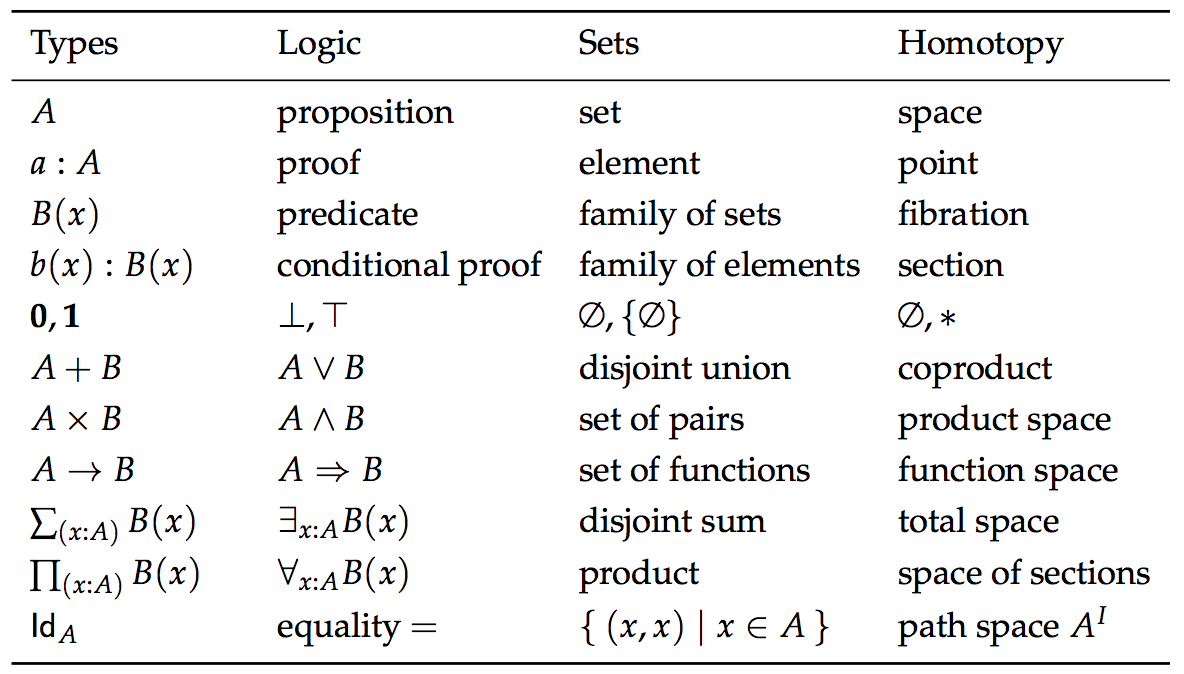
\includegraphics[scale=0.47]{images/hott}
  \end{center}
  \footnotetext[4]{\url{https://hott.github.io/book/nightly/hott-online-1186-gee8923a.pdf\#page=23}}
\end{frame}

\begin{frame}{The Elephant}
  \begin{center}
    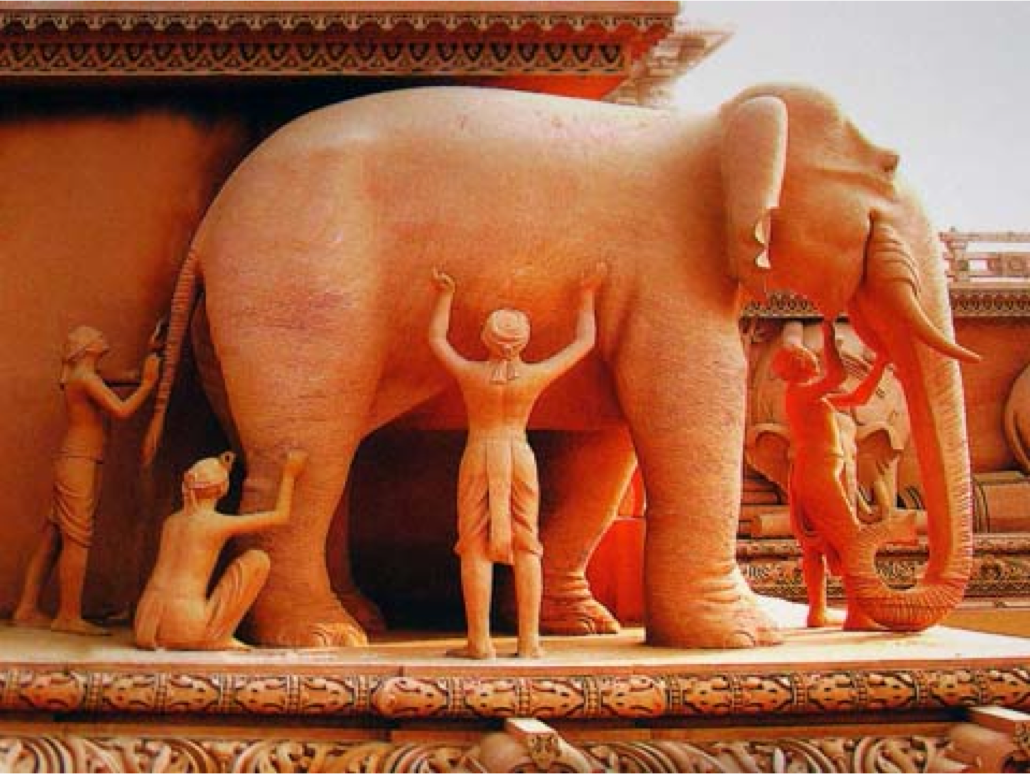
\includegraphics[scale=0.28]{images/elephant}
  \end{center}
\end{frame}

\begin{frame}[fragile]{Let's Prove Some Theorems!}
  \begin{outline}
    \1 Modus Ponens: $a \Rightarrow (a \Rightarrow b) \Rightarrow b$
    \1 Modus Tollens: $\neg{b} \Rightarrow (a \Rightarrow b) \Rightarrow \neg{a}$
    \1 Ex Falso Quodlibet: $\bot \Rightarrow a$
    \1 Eagle: $(a \Rightarrow d \Rightarrow c) \Rightarrow a \Rightarrow (b \Rightarrow e \Rightarrow d) \Rightarrow b \Rightarrow e \Rightarrow c$
    \1 Batman: $\neg{\neg{\neg{a}}} \Rightarrow \neg{a}$
    \pause
    \\~\
    \\~\
    \begin{minted}[escapeinside=@@,mathescape=true]{Lean}
def modus_ponens : a → (a → b) → b := sorry

def modus_tollens : (b → empty) → (a → b) → (a → empty) := sorry

def ex_falso_quodlibet : empty → a := sorry

def eagle : (a → d → c) → a → (b → e → d) → b → e → c := sorry

def batman : (((a → empty) → empty) → empty) → (a → empty) := sorry
    \end{minted}
  \end{outline}
\end{frame}

\begin{frame}{Principle of Explosion}
  \begin{center}
    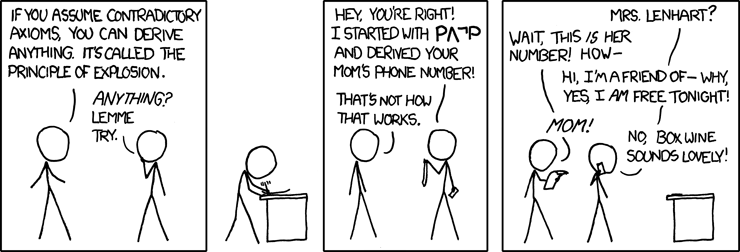
\includegraphics[scale=0.48]{images/principle_of_explosion}
  \end{center}
\end{frame}

\begin{frame}[fragile]{Why total functions?}
  \begin{outline}
    \1 Haskell, being a practical programming language, allows non-total functions and because of that is logically inconsistent
    \1 To see why consider the function
    \\~\
    \begin{minted}[escapeinside=@@,mathescape=true]{Haskell}
fix :: (a -> a) -> a
fix f = f (fix f)
    \end{minted}
    \pause
    \1 Lean disallows such definitions and even just assuming that such function exists yields a contradiction
    \\~\
    \begin{minted}[escapeinside=@@,mathescape=true]{Lean}
variable fix {a : Type} : (a → a) → a

def wtf : empty := sorry
    \end{minted}
    \1 Can you see how?
  \end{outline}
\end{frame}

\begin{frame}[fragile]{Function extensionality}
  \begin{outline}
    \begin{minted}[escapeinside=@@,mathescape=true]{Lean}
def funext {f g : a → b} (h : Π x, f x = g x) : f = g
    \end{minted}
    \pause
    \1 Let's use it to prove:
    \\~\
    \begin{minted}[escapeinside=@@,mathescape=true]{Lean}
def foo : (@$\lambda$@ x, 2 * x) = (@$\lambda$@ x, x + x) := sorry
    \end{minted}
  \end{outline}
\end{frame}

\begin{frame}[fragile]{Isomorphisms}
  \begin{minted}[escapeinside=@@,mathescape=true]{Lean}
structure iso (a b : Type) :=
(f : a → b) (g : b → a) (gf : Π x, g (f x) = x) (fg : Π x, f (g x) = x)

def inv {a b} : iso a b → iso b a := sorry

def comp {a b c} : iso a b → iso b c → iso a c := sorry
  \end{minted}
\end{frame}

\begin{frame}[fragile]{Equivalences}
  \begin{minted}[escapeinside=@@,mathescape=true]{Lean}
def fiber {a b} (f : a → b) (y : b) := @$\Sigma$@ x : a, f x = y

def iscontr (a : Type) := @$\Sigma$@ x : a, Π y : a, x = y

structure eqv (a b : Type) :=
(f : a → b) (h : Π y : b, iscontr (fiber f y))
  \end{minted}
\end{frame}

\begin{frame}[fragile]{Kan Extensions}
  \begin{minted}[escapeinside=@@,mathescape=true]{Lean}
def ran (g h : Type → Type) (a : Type) := Π b, (a → g b) → h b

def lan (g h : Type → Type) (a : Type) := @$\Sigma$@ b, (g b → a) × h b
  \end{minted}
\end{frame}

\begin{frame}[fragile]{Perfectly Balanced Trees}
  \begin{minted}[escapeinside=@@,mathescape=true]{Lean}
inductive F (g : Type → Type) : Type → Type 1
| F0 : Π {a}, a → F a
| F1 : Π {a}, F (g a) → F a

inductive G (a : Type) : Type
| G0 : a → G
| G1 : a → G → G

inductive G23 (a : Type) : Type
| G2 : a → a → G23
| G3 : a → a → a → G23
  \end{minted}
\end{frame}

\begin{frame}[fragile]{Perfectly Balanced Trees (continued)}
  \begin{minted}[escapeinside=@@,mathescape=true]{Lean}
def iter {a} (g : a → a) : @$\mathbb{N}$@ → a → a
| 0 := id
| (n + 1) := iter n @$\circ$@ g

def S (g : Type → Type) (a : Type) := @$\Sigma$@ n : @$\mathbb{N}$@, iter g n a

def sf_iso {g a} : iso (S g a) (F g a) := sorry
  \end{minted}
\end{frame}

\begin{frame}[fragile]{Haskell Core Language}
  \begin{minted}[escapeinside=@@,mathescape=true]{Haskell}
data Expr b
  = Var   Id
  | Lit   Literal
  | App   (Expr b) (Arg b)
  | Lam   b (Expr b)
  | Let   (Bind b) (Expr b)
  | Case  (Expr b) b Type [Alt b]
  | Tick  (Tickish Id) (Expr b)
  | Type  Type
  | Cast  (Expr b) Coercion
  | Coercion Coercion

data Type
  = TyVarTy   Var
  | LitTy     TyLit
  | AppTy     Type Type
  | ForAllTy  !TyCoVarBinder Type
  | FunTy     Type Type
  | TyConApp  TyCon [KindOrType]
  | CastTy    Type KindCoercion
  | CoercionTy Coercion
  \end{minted}
\end{frame}

\begin{frame}[fragile]{Lean Core Language}
  \begin{minted}[escapeinside=@@,mathescape=true]{Lean}
inductive expr
| var         : nat → expr
| sort        : level → expr
| const       : name → list level → expr
| mvar        : name → name → expr → expr
| local_const : name → name → binder_info → expr → expr
| app         : expr → expr → expr
| lam         : name → binder_info → expr → expr → expr
| pi          : name → binder_info → expr → expr → expr
| elet        : name → expr → expr → expr → expr
| macro       : macro_def → list expr → expr
  \end{minted}
\end{frame}

\begin{frame}{Example of Practical Applications: Crypto Algorithms}
  \begin{outline}
    \1 \textbf{HACL*}\footnotemark[5] is a formally verified cryptographic library in F*
    \1 {\em HACL} stands for High-Assurance Cryptographic Library
    \1 The goal of this library is to develop verified C reference implementations for popular cryptographic primitives and to verify them for memory safety, functional correctness, and secret independence
    \1 The resulting generated C code is used in Mozilla Firefox and Wireguard
    \footnotetext[5]{\url{https://github.com/project-everest/hacl-star}}
  \end{outline}
\end{frame}

\begin{frame}{``The Relation of Mathematics and Physics''\footnotemark[6] \\ by Richard Feynman}
  \small
  \begin{outline}
    \1 ``Why nature is mathematical is, again, a mystery.''
    \1 ``As people who looked at this thing as physicists cannot convert this thing to to any other language you have. If you want to discuss nature, to learn about nature, to appreciate nature, it's necessary to find out the language that she speaks in. She offers her information in only one form.''
    \1 ``To summarize, I would use the words of Jeans, who said that \textbf{"the Great Architect seems to be a mathematician"}. To those who do not know mathematics it is difficult to get across a real feeling as to the beauty, the deepest beauty, of nature. If you want to learn about nature, to appreciate nature, it is necessary to understand the language that she speaks in.''
  \end{outline}
  \footnotetext[6]{\url{http://www.cornell.edu/video/richard-feynman-messenger-lecture-2-relation-mathematics-physics}}
\end{frame}

\begin{frame}{Further reading}
  \small
  \begin{outline}
    \1 ``Theorem Proving in Lean'' \url{https://leanprover.github.io/theorem_proving_in_lean}
    \1 ``An Introduction to Lean'' \url{https://leanprover.github.io/introduction_to_lean}
    \1 ``Constructive Mathematics and Computer Programming'' by \mbox{Per Martin-L\"{o}f}
    \1 ``Proofs and Types'' by \mbox{Jean-Yves Girard}
    \1 ``Physics, Topology, Logic and Computation: A Rosetta Stone'' by \mbox{John Baez} and \mbox{Mike Stay}
    \1 ``Analytic Combinatorics'' by \mbox{Philippe Flajolet} and \mbox{Robert Sedgewick}
    \1 ``Homotopy Type Theory: Univalent Foundations of Mathematics'' by \mbox{The Univalent Foundations Program}
    \1 Code and slides from this talk: \url{https://github.com/skaslev/proofs-talk}
  \end{outline}
\end{frame}

\begin{frame}{Questions?}
\end{frame}

\end{document}
